\documentclass[11pt,a4paper]{article}
\usepackage[utf8]{inputenc}
\usepackage{geometry}
\usepackage{enumitem}
\usepackage{booktabs}
\usepackage{longtable}
\usepackage{titlesec}
\usepackage{array}
\usepackage{float}
\usepackage{graphicx}
\usepackage{amsmath}

% Page geometry
\geometry{
    left=25mm,
    right=25mm,
    top=25mm,
    bottom=25mm
}

% Formatting for sections
\titleformat{\section}{\normalfont\large\bfseries}{\thesection.}{0.5em}{}
\titlespacing*{\section}{0pt}{1.5ex plus 1ex minus .2ex}{1ex plus .2ex}

\begin{document}

\begin{center}
    \textbf{\Large FORMAT FOR SUBMITTING ANNUAL REPORT ON RESPOND PROJECTS}
\end{center}

\vspace{1em}

\noindent \textbf{Period of Report:} 01.03.2025 TO 28.01.2026 \\
\textbf{Annual Report No.:} First (Consolidated)

\begin{enumerate}[label=\textbf{\arabic*.}]
    \item \textbf{Title of Research Project:} Utilizing satellite based-observations to correct the CMIP6 climate projections of sea level anomaly and significant wave height

    \item \textbf{Name \& Designation of the Principal Investigator:} Dr. Pritam Anand, Assistant Professor \\
    \textbf{Name \& address of the institution:} Dhirubhai Ambani University, Nr Reliance Cross road, Gandhinagar, 382007

    \item \textbf{DOS sanction order No. and date:} RAC- S/FRP/24-25/03, Date 21-01-2025

    \item \textbf{Starting date of the Project:} 21-01-2025

    \item \textbf{Grants approved:} Rs. 2,49,860.00

    \item \textbf{Expenditure incurred during the period of project:} Rs. 5,16,890.00

    \begin{table}[h!]
        \centering
        \begin{tabular}{|p{0.3\textwidth}|p{0.3\textwidth}|p{0.3\textwidth}|}
            \hline
            \textbf{Amount approved By ISRO} & \textbf{Amount Spent} & \textbf{Remarks if any} \\
            \hline
            (See Note Below) & 5,16,890.00 & JRF Salary (March 2025 -- Jan 2026) \\
            \hline
        \end{tabular}
    \end{table}

    \item \textbf{Staff Salaries:} Rs. 5,16,890.00

    \item \textbf{Research Staff:}
    \begin{enumerate}[label=(\alph*)]
        \item \textbf{Name:} Shyam Saktawat \\
        \textbf{Designation:} Jr. Research Fellow \\
        \textbf{Date of appointment:} 01-03-2025
    \end{enumerate}

    \item \textbf{Project Asst/Tech Asstt:} NA

    \item \textbf{Other Staff:} NA

    \item \textbf{Equipment / Name \& Cost details:} NIL
    \begin{table}[h!]
        \centering
        \begin{tabular}{|p{0.3\textwidth}|p{0.2\textwidth}|p{0.2\textwidth}|p{0.15\textwidth}|}
            \hline
            \textbf{Item / Equipment} & \textbf{Amount approved} & \textbf{Amount spent} & \textbf{Remarks} \\
            \hline
            NIL & 0.00 & 0.00 & - \\
            \hline
        \end{tabular}
    \end{table}

    \item \textbf{Travel:} Rs. 11,000.00 (Released) / Rs. 0.00 (Spent)

    \item \textbf{Contingency:} Rs. 6,567.00 (Released) / Rs. 0.00 (Spent)

    \item \textbf{Others:} Rs. 11,000.00 (Released) / Rs. 0.00 (Spent)

    \item \textbf{Total unspent amount (Closing Balance):} Rs. 2,02,870.00

    \item \textbf{Details of grants required for 8 months:} Total: Rs. 4,99,720/-

    \begin{table}[H]
        \centering
        \begin{tabular}{|p{0.4\textwidth}|p{0.25\textwidth}|p{0.25\textwidth}|}
            \hline
            \textbf{Item} & \textbf{Amount requested now} & \textbf{Remarks} \\
            \hline
            17. Staff Salaries & Rs. 3,75,920/- & - \\
            18. Equipments & NA & - \\
            19. Miscellaneous & Rs. 13,133/- & - \\
            20. Travel & Rs. 22,000/- & - \\
            21. Institute overhead & Rs. 66,667/- & - \\
            22. Others & Rs. 22,000/- & - \\
            \hline
            \textbf{Total} & \textbf{Rs. 4,99,720/-} & - \\
            \hline
        \end{tabular}
    \end{table}

    \item \textbf{Report of the Work done:} Report is attached as Appendix.
    \\[0.25em]
    i) Objectives \\
    \textbullet\ ii) Summary of the work done \\
    \textbullet\ iii) Details of work done and results obtained during the period of the report \\
    \textbullet\ iv) Work proposed to be done during the next year

    \item \textbf{Any other relevant information:} NIL
\end{enumerate}

\vspace{3em}
\noindent \textbf{Signature of the Principal Investigator:} \\[2em]
\noindent \rule{6cm}{0.4pt} \\
(Dr. Pritam Anand)

\newpage
\appendix
\begin{center}
    \textbf{\LARGE COMPREHENSIVE PROGRESS REPORT} \\[1em]
    \textbf{\large Utilizing Satellite-based Observations to Correct CMIP6 Climate Projections of Sea Level Anomaly and Significant Wave Height} \\[1em]
    \textbf{ISRO Research Grant Project}
\end{center}

\vspace{1em}
\noindent \textbf{Principal Investigator:} Dr. Pritam Anand \\
\textbf{JRF:} Shyam Saktawat \\
\textbf{Institution:} Dhirubhai Ambani University (DAU) \\
\textbf{Reporting Period:} March 2025 - February 2028 \\
\textbf{Current Report Period:} 01.03.2025 - 28.01.2026

\section*{i) Objectives}
Earth System Models can show systematic errors because of parameterizations, grid resolution and limitations in representing complex ocean–atmosphere processes. The objective of this work is to quantify these uncertainties in CMIP6 projections of Significant Wave Height (SWH) and Sea Level Anomaly (SLA) using satellite altimetry during the observed period (2015--2023), and to develop a data-driven correction framework to improve the projections used for applications.

\begin{enumerate}[label=\alph*)]
    \item Quantify uncertainties in CMIP6 projections of SWH and SLA during the observed period (2015--2023) using merged multi-mission altimeter products.
    \item Develop and validate an AI/ML-based bias correction model to correct systematic model errors in CMIP6 datasets.
    \item Generate probabilistic long-term forecasts with improved reliability for SWH and SLA over the Indian Ocean using corrected CMIP6 projections under SSP scenarios.
\end{enumerate}

\noindent\textbf{Relevance:} Accurate projections of sea level and wave climate are important for coastal planning and hazard assessments (storm surge and coastal flooding). Using multi-mission altimetry (including SARAL/AltiKa) helps us evaluate model performance and build corrections that are directly useful for decision making.

\section*{ii) Summary of the work done}
During the reporting period (March 2025--January 2026), we focused on building the data foundation needed for uncertainty assessment and bias correction, and then running pilot studies to show the approach works. Multi-mission satellite altimetry datasets were compiled and organized for both SLA and SWH, and CMIP6 model outputs were acquired for the corresponding variables and scenarios. A processing workflow was set up to harmonize time resolution (monthly means), ensure consistent units/conventions, and generate analysis-ready datasets.

The pilots show that CMIP6 has measurable biases for SWH and SLA, and that an ML-based correction can reduce those errors compared to altimetry. The SLA pilot also confirmed that we can handle curvilinear model grids and still run the correction reliably.

\section*{iii) Details of work done and results obtained during the period of the report}

\subsection*{1. Data collection and preparation}
The first phase of work focused on acquiring and organizing observational and model datasets, and preparing them for analysis. The compiled inventory includes long-term satellite altimetry records (from 1992 onwards) and CMIP6 historical/scenario simulations, with emphasis on the 2015--2023 overlap period for evaluation and training.

\textbf{a) Satellite Altimetry (Observation):}
Gridded Level-4 (L4) merged products for SLA and SWH were acquired from Copernicus/AVISO repositories (nominal $\sim$25\,km spatial resolution). The merged product integrates measurements from multiple missions, including SARAL/AltiKa, Jason series, Sentinel-3 series, Sentinel-6, Cryosat-2, and other contributing platforms. These products provide consistent, quality-controlled fields suitable for climate-scale evaluation of model biases.
\begin{itemize}
    \item \textbf{Missions:} SARAL/AltiKa, Jason-3, Sentinel-3A/B, Sentinel-6A, Cryosat-2, and Haiyang-2B.
    \item \textbf{Coverage:} Global coverage; pilot focus on the Indian Ocean sector (50$^\circ$E--110$^\circ$E, 70$^\circ$S--70$^\circ$N).
    \item \textbf{Temporal handling:} Monthly means were used to match CMIP6 ocean output frequency and to reduce high-frequency sampling noise.
\end{itemize}

\textbf{b) CMIP6 Climate Models (Input):}
CMIP6 historical simulations and SSP scenario outputs were obtained from ESGF, including representative models used for pilot testing. For SLA, the sea surface height variable (\texttt{zos}) was converted to an anomaly by removing the long-term mean reference.
\begin{itemize}
    \item \textbf{Models:} MPI-ESM1-2-LR, ACCESS-ESM1-5, CESM2.
    \item \textbf{Variables:} \texttt{zos} (sea surface height above geoid) and SWH (significant wave height).
\end{itemize}

\subsection*{2. Significant Wave Height (SWH): bias assessment and ML correction}

\textbf{Significance of Biases:}
An initial pilot analysis over the Indian Ocean (2015--2020) quantified the discrepancy between raw CMIP6 SWH output and satellite altimetry. The regional mean difference (model minus satellite) was approximately +0.162\,m, with larger biases in specific sub-regions. This confirms that bias correction is required before using model projections for applications.

\textbf{ML Correction Methodology:}
To correct these systematic errors, a Random Forest regression model was trained to learn the mapping from the raw model state to the satellite-observed value. The model inputs were: raw model SWH, latitude, longitude, and a cyclic representation of month (seasonality). The model target was the satellite SWH. For the pilot demonstration, the training period was 2015--2018 and the independent evaluation period was 2019--2020, consistent with the proposal's emphasis on separating training and validation windows.

\begin{figure}[H]
    \centering
    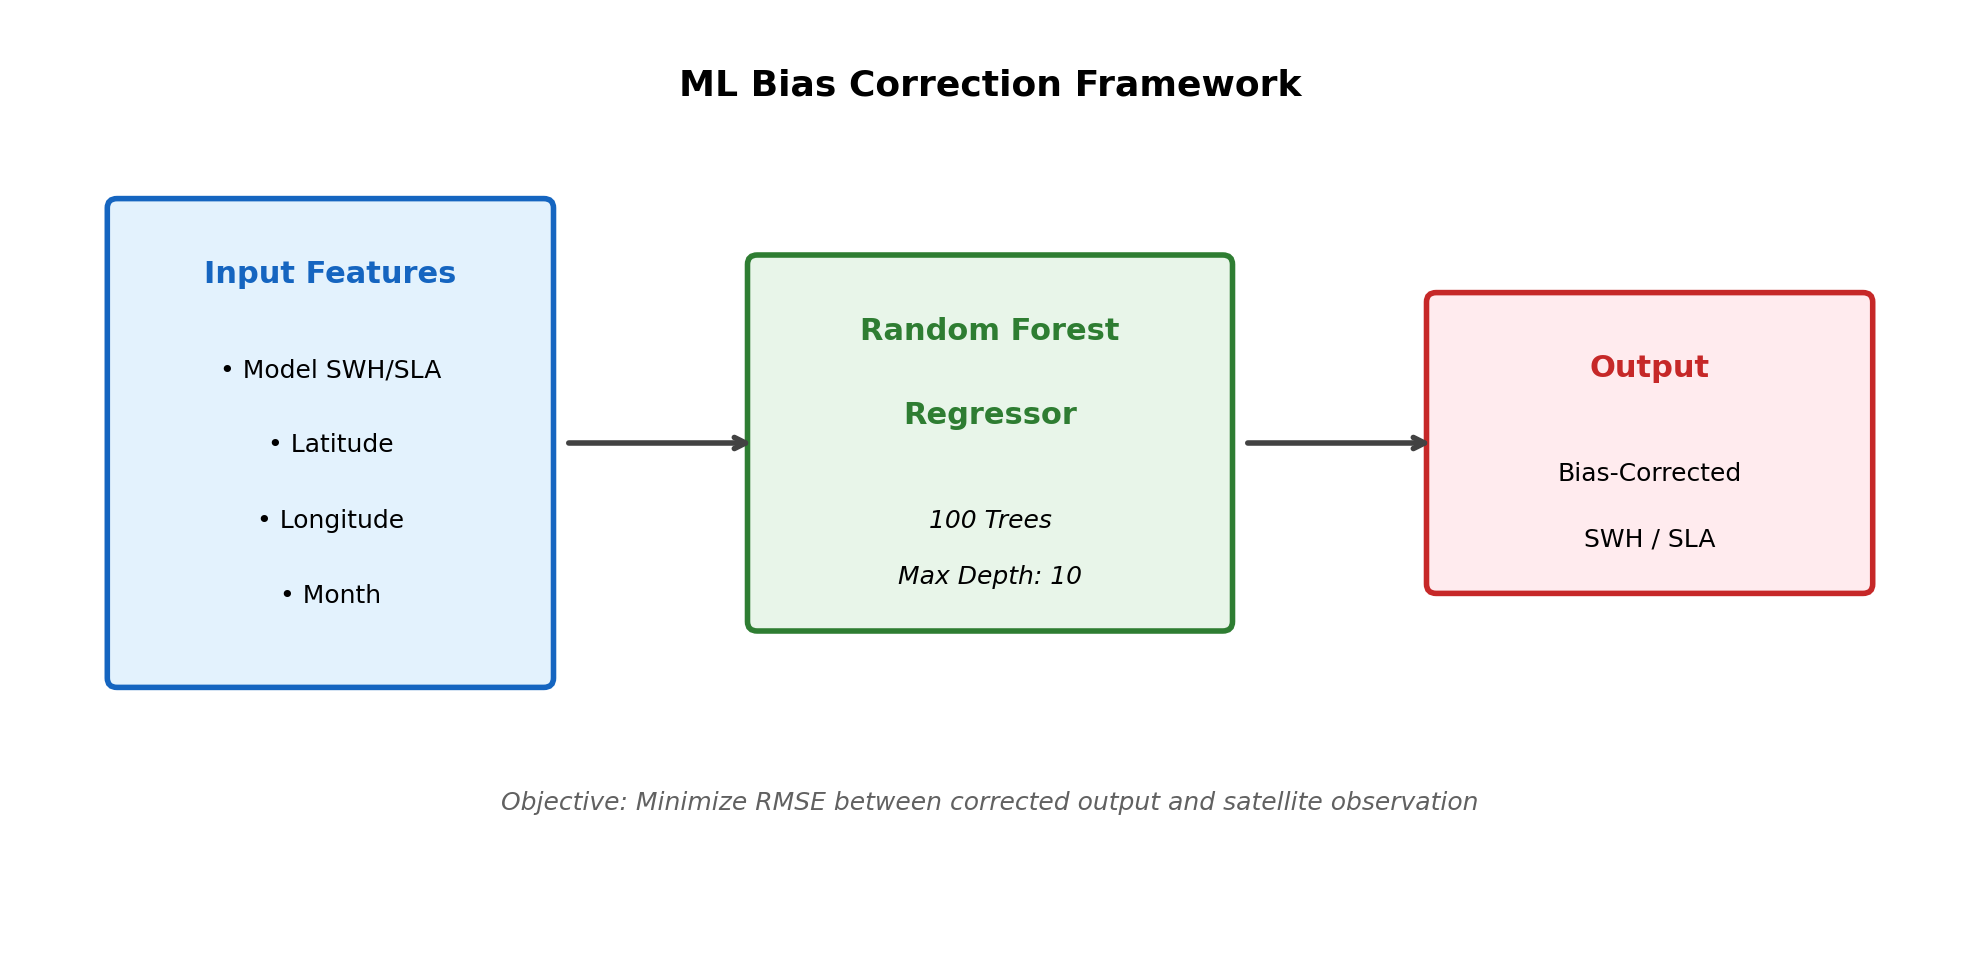
\includegraphics[width=0.95\textwidth]{report_diagrams/model_schema.png}
    \caption{Bias correction model inputs and outputs (Random Forest regressor).}
    \label{fig:ml_model}
\end{figure}

\textbf{Results:}
The correction model reduced the SWH error substantially on the independent test period. The RMSE decreased from 0.599\,m (raw CMIP6) to 0.308\,m (bias-corrected), corresponding to an improvement of approximately 48\%. The corrected estimates align more closely with the 1:1 relationship in scatter space and reproduce the observed temporal variability in regional averages (Fig.~\ref{fig:swh_results}).

\begin{figure}[H]
    \centering
    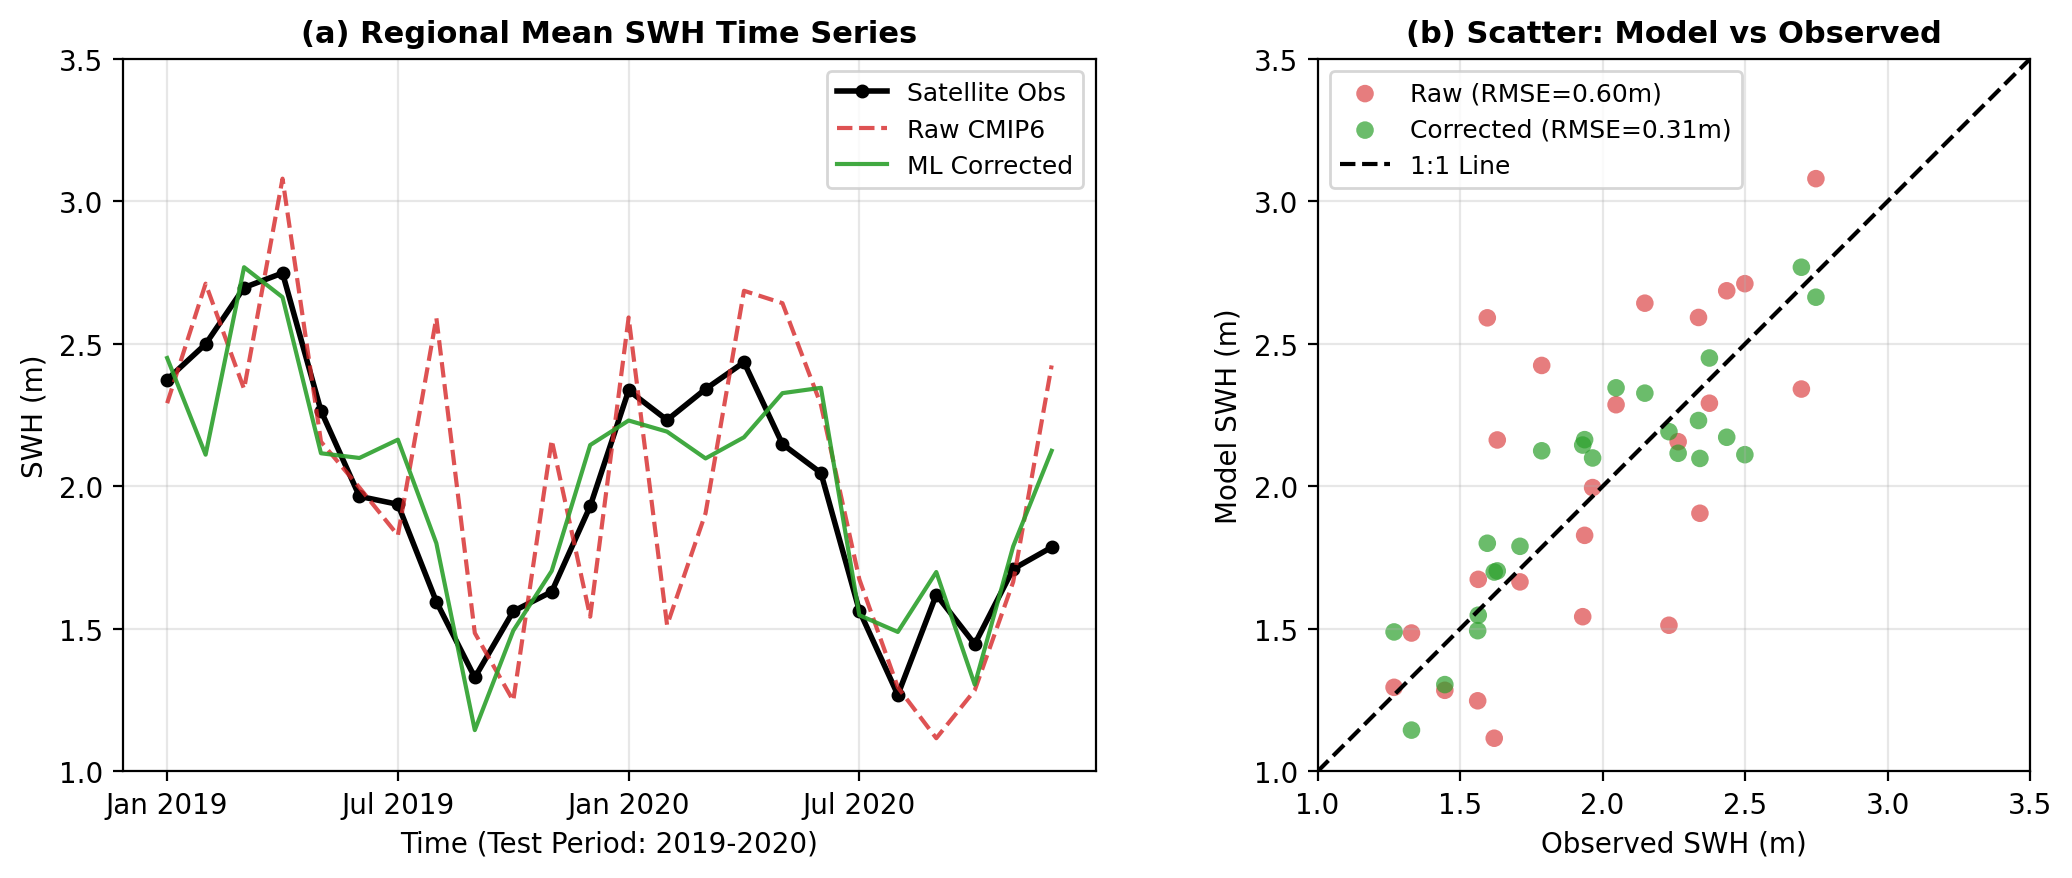
\includegraphics[width=0.95\textwidth]{plots/swh_results_combined.png}
    \caption{SWH bias correction results for the Indian Ocean pilot region (2019--2020 test period).}
    \label{fig:swh_results}
\end{figure}

\subsection*{3. Sea Level Anomaly (SLA): pilot correction results}
The SLA workflow was tested in a high-latitude pilot region (63$^\circ$N--79$^\circ$N, 50$^\circ$E--108$^\circ$E) to verify robustness under challenging conditions (complex coastline and potential ice contamination). A practical issue in CMIP6 ocean output is the presence of curvilinear grids. For the pilot, the model field was regridded onto the rectilinear satellite grid using a nearest-neighbour approach based on \texttt{cKDTree}. The ML correction was then applied on the aligned grid.

\textbf{Methodological Innovation:}
The pilot established a repeatable procedure for transforming model \texttt{zos} to an SLA anomaly, aligning model and satellite grids, and training the correction model. This gives a clear path to scale the workflow to the target domain.

\textbf{Results:}
\begin{itemize}
    \item \textbf{RMSE Reduction:} 0.1037m (Raw) $\to$ 0.0578m (Corrected).
    \item \textbf{Improvement:} \textbf{44.3\%} reduction in error variance.
    \item The time series analysis (Fig. \ref{fig:sla_results}) confirms that the ML model effectively corrects phase lags and amplitude mismatches in the seasonal cycle.
\end{itemize}

\begin{figure}[H]
    \centering
    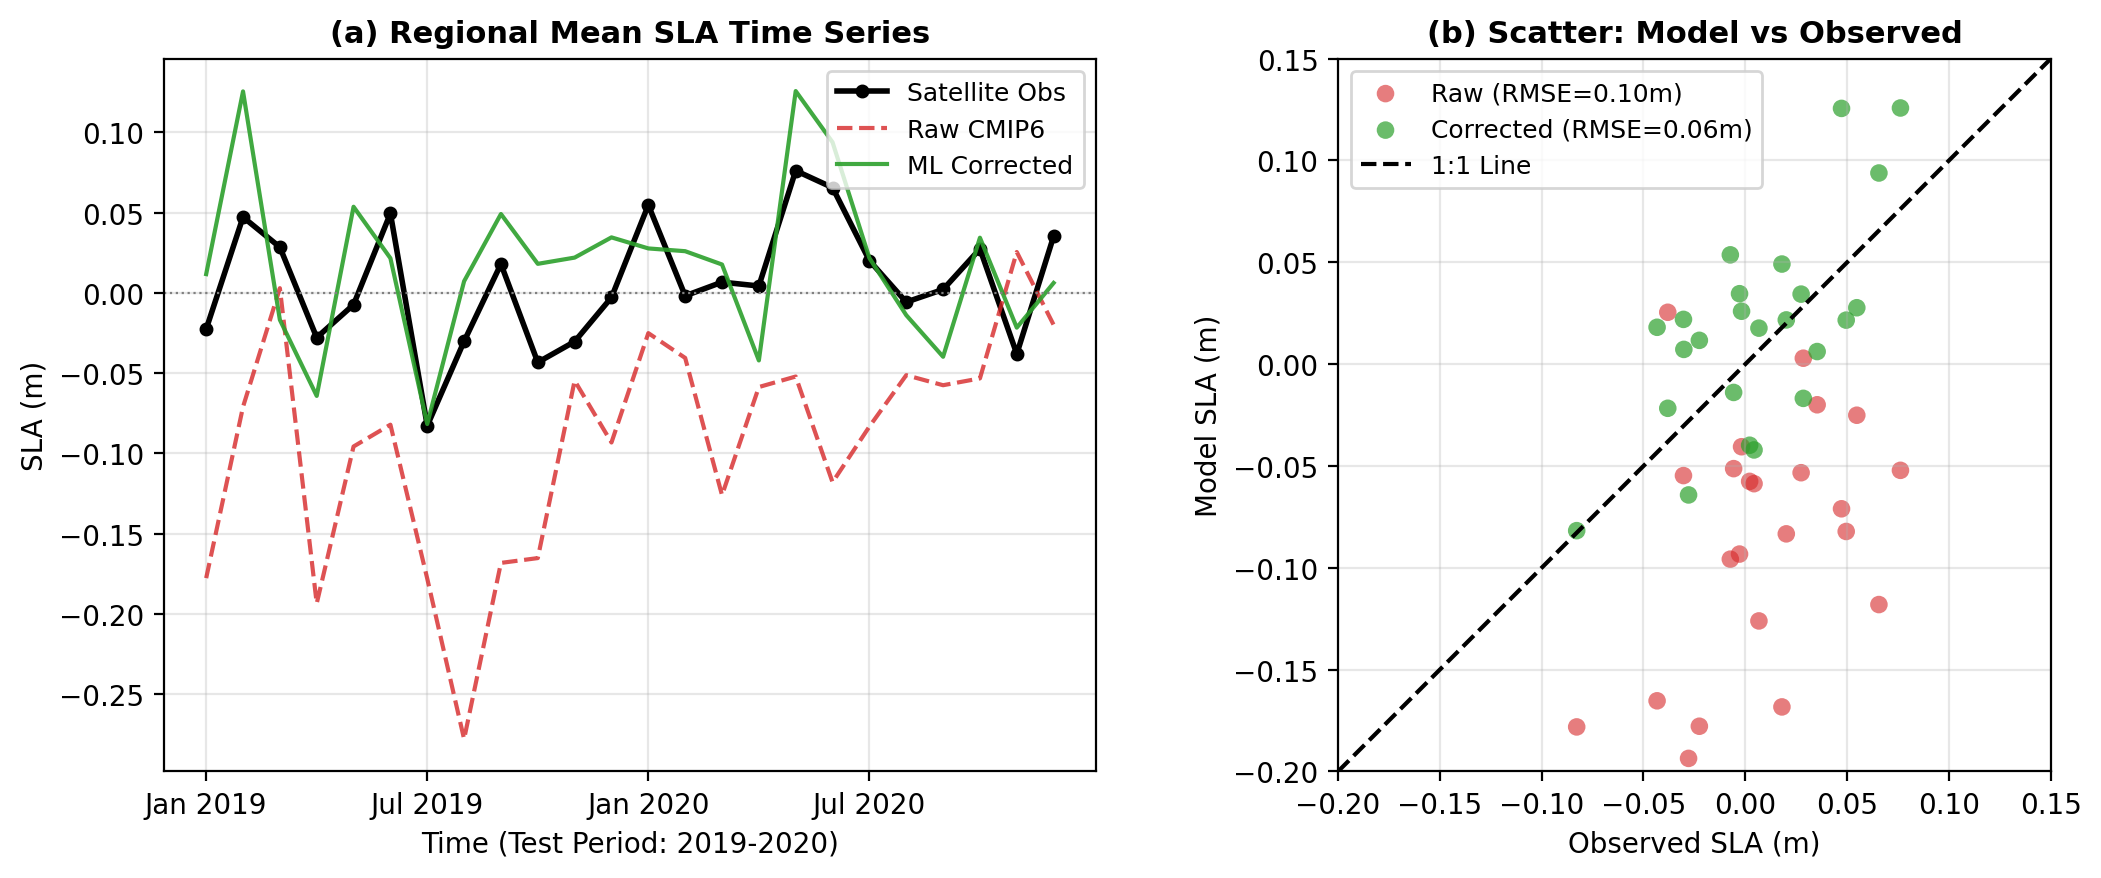
\includegraphics[width=0.95\textwidth]{sla_plots/sla_results_combined.png}
    \caption{SLA bias correction results for the high-latitude pilot region (2019--2020 test period).}
    \label{fig:sla_results}
\end{figure}

\section*{iv) Work proposed to be done during the next year}
The next phase of work will prioritize scaling from pilots to a production-ready workflow:
\begin{itemize}
    \item \textbf{Data processing at scale:} Complete systematic preprocessing for the full observed overlap window (2015--2023) across the Indian Ocean for SLA and SWH, including consistent gridding, monthly aggregation, and QC flags.
    \item \textbf{Uncertainty modelling:} Implement and benchmark probabilistic models described in the proposal (e.g., DeepAR, QRNN, Bayesian/ensemble approaches) to estimate prediction intervals and quantify uncertainty beyond point corrections.
    \item \textbf{Model evaluation:} Formalize evaluation metrics (RMSE, bias, skill scores, coverage probability and interval width for probabilistic forecasts) and compare CMIP6 model performance across sub-regions.
    \item \textbf{Re-computing projections:} Apply validated correction models to CMIP6 SSP scenario projections and prepare corrected datasets and documentation for sharing with ISRO.
\end{itemize}

\end{document}
